\section{Markov Random Fields}
\label{sec:mrf_intro}

\subsection{Boltzmann distributions}
Boltzmann (or Gibbs) distributions are one of the fundamental mathematical formalisms connecting statistical physics with probabilistic modeling and machine learning. They describe the probability of a configuration of a system in equilibrium as a function of its energy and temperature, and thus provide a natural framework for representing random processes that favor low-energy, or equivalently low-cost, states. For a configuration $x \in \mathcal{X}$ and energy function $E(x)$, the Boltzmann distribution at inverse temperature $\beta = 1/T$ is
\begin{equation}
    \label{equ:boltzmann_distribution}
    p_\beta(x) = \frac{1}{Z(\beta)} \exp\!\left(-\beta\,E(x)\right), \qquad 
    Z(\beta) = \sum_{x\in\mathcal{X}} \exp\!\left(-\beta\,E(x)\right),
\end{equation}
where $Z(\beta)$ is the \emph{partition function}, a normalization constant ensuring that $p_\beta$ is a valid probability distribution. The role of $Z(\beta)$ is crucial both in physics and in probabilistic modeling, since it encodes the relationship between microscopic configurations and macroscopic quantities such as free energy and entropy. However, its computation requires summation over all possible states, which becomes intractable in high dimensions and is a central difficulty in applying Boltzmann distributions to complex systems.

The behavior of $p_\beta$ interpolates smoothly between two extremes: as $\beta \to 0$ (high temperature), all states become equally likely and the distribution approaches the uniform distribution on $\mathcal{X}$; as $\beta \to \infty$ (low temperature), the distribution concentrates on the minimizers of $E(x)$, corresponding to ground states of the system. This property provides a powerful conceptual bridge to combinatorial optimization, where feasible solutions can be interpreted as states and the objective function as an energy: minimizing $E(x)$ corresponds to finding the most probable state at low temperature. Simulated annealing \citep{kirkpatrick_optimization_1983}, a classical stochastic optimization algorithm, exploits this principle by gradually decreasing the temperature to bias sampling toward global optima while avoiding poor local minima.

From an information-theoretic perspective, Boltzmann distributions also arise as the maximum-entropy distribution subject to a constraint on expected energy \citep{jaynes_information_1957}. This general principle explains their ubiquity: whenever only limited information about a system is available, such as the average energy, the Gibbs distribution is the least biased model consistent with that knowledge. This dual interpretation, as both a physical law and a statistical modeling tool, explains their central role in probabilistic inference and machine learning.

Applications of Boltzmann distributions are widespread. In computer vision, they were introduced to model images through Markov Random Fields, leading to the pioneering use of stochastic relaxation for Bayesian image restoration \citep{geman_stochastic_1984}. In machine learning, they underlie Boltzmann machines and their restricted variants, which learn distributed representations via energy-based training \citep{hinton_reducing_2006}. More broadly, the formalism provides the probabilistic foundation for modern energy-based models, where designing an appropriate energy function defines the distribution over structured objects such as graphs, sequences, or combinatorial configurations.

In summary, Boltzmann distributions encapsulate the idea that structured solutions to optimization and inference problems can be modeled as outcomes of a random process governed by an energy function. They provide a rigorous link between optimization, statistical physics, and information theory, while also highlighting the computational challenges associated with the partition function. This background sets the stage for the use of Boltzmann-type models in subsequent chapters to represent and solve combinatorial optimization problems.


\paragraph{Exponential-family form and learning.}
A large class of energy-based models, including Markov Random Fields, can be expressed within the general framework of exponential families. In this setting, a distribution over configurations $x \in \mathcal{X}$ is written as

\begin{equation}
p_\theta(x) = \exp\!\left(\theta^\top \phi(x) - A(\theta)\right),
\end{equation}

where $\phi(x)$ is a vector of sufficient statistics, $\theta$ is the vector of natural parameters, and $A(\theta)=\log \sum_{x\in\mathcal{X}} \exp(\theta^\top \phi(x))$ is the log-partition function. This formulation generalizes the Boltzmann distribution by emphasizing the role of feature functions $\phi(x)$, which capture local interactions or structural properties of $x$. The log-partition function $A(\theta)$ ensures normalization and is also the cumulant-generating function of the sufficient statistics, which implies convexity and well-behaved optimization landscapes for maximum likelihood estimation \citep{wainwright_graphical_2007}.

Learning in exponential-family models typically proceeds by maximum likelihood, which requires computing gradients of the log-likelihood with respect to $\theta$. For a dataset $\mathcal{D}=\{x^{(1)},\dots,x^{(N)}\}$, the gradient takes the moment-matching form
\begin{equation}
\nabla_\theta \log p_\theta(\mathcal{D}) = \sum_{i=1}^N \phi(x^{(i)}) - N \,\mathbb{E}_{p_\theta}[\phi(X)].
\end{equation}
This expression highlights the core difficulty: while the first term (empirical sufficient statistics) is easily computed from data, the second term requires expectations under the model distribution, which are generally intractable due to the partition function. As a result, practical learning algorithms must resort to approximate inference schemes. Classical approaches include Monte Carlo methods such as Gibbs sampling, which generate approximate samples from $p_\theta$, and variational approximations that replace $A(\theta)$ with a tractable surrogate. More recently, amortized inference networks and neural variational methods have been proposed to approximate the intractable expectations efficiently \citep{wiseman_amortized_2019}.

\begin{example}{\hrule\vspace{.2em}Boltzmann Machine (pairwise EBM)\vspace{.2em}\hrule}
A canonical example of an exponential-family energy-based model is the Boltzmann Machine, originally developed for learning distributed representations of data. For binary variables (spins) $s_i \in \{-1,+1\}$, the energy is defined by pairwise couplings and local biases:
\begin{equation}
E(s) = -\sum_{(i,j)\in E} w_{ij} s_i s_j - \sum_i \theta_i s_i. \label{equ:bm_energy}
\end{equation}
The corresponding distribution is
\begin{equation}
p(s) \propto \exp\!\left(\sum_{(i,j)} w_{ij} s_i s_j + \sum_i \theta_i s_i\right).
\end{equation}
Here the sufficient statistics $\phi(x)$ are the pairwise products $(s_i s_j)$ and the unary states $(s_i)$, and the natural parameters $\theta$ are the weights $w_{ij}$ and biases $\theta_i$. Learning in Boltzmann Machines requires adjusting the parameters so that the model statistics match the empirical statistics of the training data. Because the model expectations are not analytically available, training algorithms alternate between gradient updates and approximate sampling from the current model, typically using Gibbs sampling or contrastive divergence \citep{hinton_reducing_2006}. This example illustrates both the expressive power of exponential-family EBMs and the computational obstacles posed by their normalization constants.
\end{example}




\subsubsection{Sampling from Boltzmann distributions}
Because the partition function $Z(\beta)$ grows exponentially with the size of the configuration space, direct sampling from Boltzmann distributions is intractable in all but the most trivial cases. To address this, approximate methods based on Monte Carlo simulation are employed. The general principle is to design a stochastic process whose stationary distribution coincides with the desired Boltzmann distribution $p_\beta$, and then to generate approximate samples by simulating this process. This class of approaches, known as Markov Chain Monte Carlo (MCMC), has been foundational both in statistical physics and in probabilistic inference for graphical models \citep{metropolis_monte_1949,hastings_monte_1970,geman_stochastic_1984}.

The most classical algorithm is the Metropolis--Hastings method, which iteratively proposes a new state $x'$ from a distribution $q(x'|x)$ conditioned on the current state $x$, and accepts or rejects it with a probability that depends on the energy difference $E(x')-E(x)$. This mechanism guarantees that the resulting Markov chain satisfies detailed balance, ensuring convergence to $p_\beta$. A related but more specialized method is Gibbs sampling, which leverages the conditional structure of Markov Random Fields: each variable is updated in turn by drawing from its conditional distribution given its neighbors, leading to particularly simple update rules in models such as the Ising or Potts models. Both of these approaches have been extensively used in applications ranging from Bayesian image restoration \citep{geman_stochastic_1984} to the training of Boltzmann machines \citep{hinton_reducing_2006}.

Beyond these classical methods, a variety of other strategies have been explored. Importance sampling reuses samples from a simpler distribution $q(x)$ by reweighting them according to $p_\beta(x)/q(x)$. Although conceptually straightforward, its effectiveness deteriorates rapidly in high-dimensional spaces when $q$ and $p_\beta$ differ significantly. More advanced approaches include tempered and parallel MCMC schemes, which simulate multiple chains at different temperatures to help traverse energy barriers, and gradient-based proposals adapted from continuous-state MCMC for use in discrete settings \citep{zanella_informed_2017,sun_path_2022,sun_stochastic_2024}. These refinements aim to improve mixing, i.e., the rate at which the chain explores the state space, which is often the main bottleneck in practice.

Despite their widespread use, sampling methods face significant limitations when applied to discrete, high-dimensional distributions of combinatorial nature. Energy landscapes associated with such problems are often rugged and multimodal, with many local optima separated by high-energy barriers. In these settings, naive MCMC chains can exhibit \emph{slow mixing}, meaning they require an impractically large number of iterations to approximate the target distribution well. This issue is particularly acute in the context of combinatorial optimization problems, where the most relevant configurations (low-energy solutions) may be extremely sparse compared to the size of the configuration space. Overcoming these difficulties remains an active research challenge and has motivated both theoretical investigations into mixing times and practical advances in algorithm design.

In this thesis, we limit ourselves here to providing this general overview of sampling methods for Boltzmann-type distributions, while postponing a deeper discussion of their limitations and adaptations to discrete combinatorial domains. These issues, including the connections between slow mixing and the structure of combinatorial optimization problems, will be revisited in later chapters once the optimization problems themselves have been formally introduced.


\paragraph{Metropolis--Hastings (MH).}
The Metropolis--Hastings algorithm is one of the most fundamental methods in Markov Chain Monte Carlo (MCMC), originally introduced in statistical physics to simulate systems of interacting particles \citep{metropolis_monte_1949,hastings_monte_1970}. Its key idea is to construct a Markov chain that explores the configuration space by proposing new states according to a user-defined distribution and then accepting or rejecting them in a way that ensures convergence to the target Boltzmann distribution $p_\beta$.

Given the current state $x$, a candidate $x'$ is proposed from a distribution $q(x'|x)$. The proposal is then accepted with probability
\begin{equation}
\alpha(x,x')=\min\!\left(1,\frac{p_\beta(x')\,q(x|x')}{p_\beta(x)\,q(x'|x)}\right)
=\min\!\left(1,\exp[-\beta\,(E(x')-E(x))]\frac{q(x|x')}{q(x'|x)}\right),
\end{equation}
and otherwise the chain remains at $x$. This rule guarantees that the Markov chain satisfies detailed balance with respect to $p_\beta$, ensuring that the stationary distribution is indeed the desired Boltzmann distribution provided the chain is also irreducible and aperiodic.

The flexibility of MH comes from the choice of proposal $q(x'|x)$. A simple and commonly used choice is a symmetric proposal (e.g., flipping a single spin or adding/removing an element from a set), in which case the acceptance ratio reduces to $\alpha(x,x')=\min\{1,\exp[-\beta(E(x')-E(x))]\}$. More sophisticated proposals, such as block updates or informed proposals that take into account gradients or problem structure \citep{zanella_informed_2017}, can dramatically improve mixing by guiding the chain towards regions of high probability. The efficiency of MH is therefore highly dependent on how well the proposal distribution matches the structure of the target distribution.

Despite its simplicity and generality, MH faces limitations when applied to high-dimensional discrete distributions. In rugged energy landscapes, small local moves can lead to chains that become trapped in local minima, resulting in very slow mixing and poor exploration of the state space. This issue is particularly acute in combinatorial optimization problems, where the number of near-optimal solutions may be large but separated by high-energy barriers. Addressing these limitations often requires designing problem-specific proposals, introducing auxiliary variables, or combining MH with techniques such as tempering or parallel chains. These strategies will be revisited in later chapters in the context of discrete combinatorial optimization.

\begin{algorithm}[htbp]
\caption{Metropolis--Hastings for EBMs}
\KwData{Energy $E$, inverse temperature $\beta$, proposal $q(\cdot|\cdot)$}
\KwResult{Samples $\{x_t\}_{t=1}^T \sim p_\beta$ (asymptotically)}
Initialize $x_0$; \For{$t=0$ {\bf to} $T-1$}{Propose $x'\sim q(\cdot|x_t)$; compute $\alpha=\min\!\big(1,\exp[-\beta(E(x')-E(x_t))]\frac{q(x_t|x')}{q(x'|x_t)}\big)$;\\
With prob.\ $\alpha$ set $x_{t+1}=x'$, else $x_{t+1}=x_t$.}
\end{algorithm}

\begin{example}{\hrule\vspace{.2em}MH on a 2-spin Ising model\vspace{.2em}\hrule}
Consider a toy Ising system with two binary spins $s_1,s_2\in\{-1,+1\}$ and energy $E(s)=-J s_1 s_2$. If $J>0$, aligned configurations $(+1,+1)$ and $(-1,-1)$ have lower energy. Suppose the proposal $q$ flips one spin uniformly at random. If the chain is currently in $(+1,+1)$ and proposes $(+1,-1)$, the move is accepted with probability $\exp(-2\beta J)$ since the energy increases by $2J$. At high temperature ($\beta$ small), such moves are frequently accepted, leading to rapid exploration; at low temperature ($\beta$ large), the chain spends most of its time in aligned states.

\begin{figure}[htbp]\centering
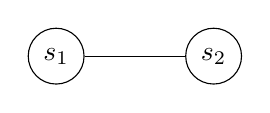
\begin{tikzpicture}[every node/.style={circle,draw}]
\node (1) at (0,0) {$s_1$}; \node (2) at (2,0) {$s_2$}; \path (1) edge (2);
\end{tikzpicture}
\caption{Two-spin Ising graph for the MH toy example.}
\end{figure}
\end{example}


\paragraph{Gibbs sampling.}
Gibbs sampling is a special case of the Metropolis--Hastings algorithm in which the proposal distribution is chosen to be the exact conditional distribution of one variable given the others. Because such proposals are always accepted, Gibbs sampling eliminates the need for an explicit acceptance step, making it one of the simplest and most widely used MCMC algorithms \citep{geman_stochastic_1984}. The method proceeds by iteratively resampling each variable $x_i$ from its conditional distribution $p(x_i \mid x_{-i})$, where $x_{-i}$ denotes all variables except $x_i$. By the Markov property of MRFs, this conditional depends only on the neighbors $N(i)$ of $i$ in the graph, which greatly reduces the computational cost in sparse models.

Gibbs sampling has several attractive features. It is easy to implement whenever conditionals are available in closed form, and in models with local interactions it naturally exploits the structure of the graph. In pairwise Markov random fields such as the Ising model, the conditional distribution of a single spin depends only on the sum of the neighboring spins, yielding a simple logistic form. Moreover, since Gibbs sampling updates one variable at a time, it can be seen as a stochastic analogue of coordinate descent in the energy landscape. These properties have made Gibbs sampling a standard inference method in fields ranging from image analysis and Bayesian networks to the training of Boltzmann machines.

Nevertheless, standard Gibbs sampling can suffer from poor mixing in high-dimensional or multimodal distributions, where single-variable updates are insufficient to traverse energy barriers efficiently. To mitigate this, several variants have been developed. \emph{Block Gibbs sampling} updates groups of variables jointly rather than individually, reducing correlations between successive samples and improving convergence in strongly coupled systems \citep{liu_monte_2001}. Another widely used extension is \emph{parallel tempering} (also known as replica exchange MCMC), where multiple chains are run at different temperatures and periodically exchange states. This approach helps overcome slow mixing in rugged energy landscapes by allowing high-temperature chains to explore broadly and low-temperature chains to refine local structure \citep{geyer_markov_1991}. These and related techniques demonstrate the adaptability of Gibbs sampling to challenging inference tasks.

A more detailed analysis of such limitations and variants, especially in the discrete and combinatorial settings central to this thesis, will be deferred to later chapters once combinatorial optimization problems have been formally introduced.

\begin{algorithm}[htbp]
\caption{Gibbs sampling}
\KwData{Factorization $\{\psi_c\}$; schedule over variables}
\KwResult{Samples $\{x_t\}$}
Initialize $x$; \For{$t=0$ {\bf to} $T-1$}{\For{each variable $i$ (in random or fixed order)}{Sample $x_i \sim p(x_i \mid x_{N(i)}) \propto \prod_{c\ni i}\psi_c(x_c).$}}
\end{algorithm}

\begin{example}{\hrule\vspace{.2em}Gibbs on a $2\times 2$ Ising grid\vspace{.2em}\hrule}
Consider four binary spins $\{s_1,s_2,s_3,s_4\}$ arranged in a square with pairwise potential $\psi(s_i,s_j)=\exp(J s_is_j)$. By the Markov property, the conditional distribution of $s_1$ given its neighbors depends only on $s_2$ and $s_3$, and is given by
\[
p(s_1=+1 \mid s_2,s_3) \propto \exp\!\big(J(s_2+s_3)\big).
\]
The Gibbs sampler cycles through the four spins, repeatedly resampling each from its conditional. Over time, the sequence of states produced by this process approximates the Boltzmann distribution of the grid.


\begin{figure}[htbp]\centering
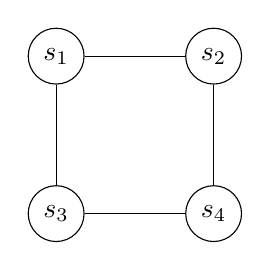
\begin{tikzpicture}[every node/.style={circle,draw}]
\node (1) at (0,0) {$s_1$}; \node (2) at (2,0) {$s_2$};
\node (3) at (0,-2) {$s_3$}; \node (4) at (2,-2) {$s_4$};
\path (1) edge (2); \path (1) edge (3); \path (2) edge (4); \path (3) edge (4);
\end{tikzpicture}\caption{$2\times 2$ Ising grid for Gibbs sampling.}\end{figure}
\end{example}


\paragraph{Importance sampling (IS).}
Classical importance sampling is a general Monte Carlo technique for estimating expectations under a complex distribution $p$ by drawing samples from a simpler proposal distribution $q$ and reweighting them. Given $x^{(i)}\sim q$, the self-normalized estimator of $\mathbb{E}_p[f(X)]$ is
\begin{equation}
\widehat{\mathbb{E}}_p[f]=\frac{\sum_{i=1}^N w^{(i)} f(x^{(i)})}{\sum_{i=1}^N w^{(i)}},\qquad w^{(i)}=\frac{p(x^{(i)})}{q(x^{(i)})}.
\end{equation}
The efficiency of IS depends critically on the quality of the proposal $q$: if $q$ does not overlap well with $p$, the variance of the estimator explodes and the effective sample size $\mathrm{ESS}=\tfrac{(\sum_i w^{(i)})^2}{\sum_i (w^{(i)})^2}$ becomes very small. For high-dimensional discrete Boltzmann distributions, constructing such good proposals is generally infeasible, which is why IS is rarely used directly in this context.

It is worth noting, however, that in the MRF literature the term ``importance sampling'' has sometimes been applied to a different family of algorithms designed for inference with evidence. In these settings, some variables are clamped to observed values and we wish to sample from the conditional distribution of the remaining free variables. One approximate strategy is to sample variables sequentially, fixing each to a value and adjusting the potentials of the factors involving it before proceeding to the next variable. This procedure can be interpreted as a form of \emph{sequential importance sampling}, where variables are generated one at a time and the distribution is updated accordingly. While the name is the same, it is important to distinguish this specialized conditional sampling from the classical IS estimator described above.

Finally, a number of extensions of IS have been proposed to make it more practical in complex models. \emph{Annealed importance sampling (AIS)} \citep{neal_annealed_1998} gradually transforms an easy-to-sample distribution into the target by introducing a sequence of intermediate distributions, while \emph{sequential importance sampling (SIS)} and related particle filtering methods \citep{doucet_sequential_2001} adapt the proposal distribution step by step as variables are sampled. These approaches are widely used in Bayesian inference and for estimating partition functions of energy-based models. Although they remain challenging to apply efficiently to large-scale combinatorial structures, they provide important conceptual links between IS and the more flexible MCMC strategies introduced earlier.

\begin{example}{\hrule\vspace{.2em}Sequential IS heuristic for MIS\vspace{.2em}\hrule}
For the Maximum Independent Set problem on a graph $G$, one may define a sequential proposal that samples vertices in some order, with probabilities biased by degree. Each time a vertex is chosen, its neighbors are excluded from further consideration, and the process continues until no more vertices can be added. The resulting independent set $S$ is feasible by construction, but biased by the sampling order. Importance weights can, in principle, be assigned to correct this bias, yielding an instance of sequential importance sampling adapted to a combinatorial constraint.
\end{example}

\paragraph{Sequential Importance Sampling (SIS).}  
In this thesis, whenever we refer to \emph{Importance Sampling} for Markov Random Fields, we specifically mean the \emph{Sequential Importance Sampling} (SIS) algorithm. Unlike the classical IS estimator that draws i.i.d.\ samples from a static proposal distribution, SIS generates samples sequentially by progressively fixing variables and adjusting the factor potentials of the remaining subproblem. This is particularly well-suited for discrete graphical models and combinatorial problems, since feasibility constraints can be enforced at each step of the sequence.  

Formally, let $X=(X_1,\dots,X_n)$ be the set of variables. SIS constructs a sequence of intermediate target distributions $p^{(1)},\dots,p^{(n)}$, where at step $t$ a variable $X_t$ is sampled conditioned on previously fixed variables. Importance weights are updated multiplicatively, correcting for proposal bias.  

\begin{algorithm}[htbp]
\caption{Sequential Importance Sampling for MRFs}
\KwData{Factor graph $H=(V,F,E)$ with potentials $\{\psi_f\}$}
\KwResult{Weighted samples $\{(x^{(i)}, w^{(i)})\}_{i=1}^N$}
\For{$i=1$ {\bf to} $N$}{
  Initialize weight $w^{(i)}=1$\;
  \For{$t=1$ {\bf to} $n$}{
    Sample $x_t^{(i)} \sim q_t(\cdot \mid x_{1:t-1}^{(i)})$\;
    Update weight 
    $w^{(i)} \gets w^{(i)} \cdot \frac{p(x_{1:t}^{(i)})}{q_t(x_t^{(i)} \mid x_{1:t-1}^{(i)})}$\;
  }
}
Normalize weights: $\tilde{w}^{(i)} = w^{(i)}/\sum_j w^{(j)}$\;
\end{algorithm}

SIS produces a weighted empirical approximation of the MRF distribution,
\[
\hat{p}(x) = \sum_{i=1}^N \tilde{w}^{(i)} \, \delta_{x^{(i)}}(x),
\]
that can be used to estimate marginals, guide greedy decoding, or construct approximate solutions. While SIS mitigates some of the difficulties of naive IS in high-dimensional discrete spaces, it remains sensitive to proposal design and can suffer from weight degeneracy, particularly when the sampling order is poorly chosen or dependencies between variables are strong \citep{doucet_sequential_2001, cappe_inference_2005}.



\subsection{Graphical models}
Graphical models provide a unifying framework for representing complex multivariate probability distributions using graphs. The central idea is that statistical dependencies among random variables can be expressed in terms of the edges of a graph, so that the global distribution factorizes into a product of local functions associated with the graph structure \citep{wainwright_graphical_2007}. This factorization makes explicit which variables interact directly and which are conditionally independent given others, allowing compact specification of high-dimensional distributions and enabling scalable inference algorithms.

Two broad families of graphical models are commonly distinguished. In \emph{directed graphical models} (also known as Bayesian networks), edges represent directed dependencies and the joint distribution factorizes into conditional probabilities along these edges. These models are well suited for encoding causal relationships and are widely used in probabilistic reasoning and learning. In \emph{undirected graphical models}, also called Markov Random Fields (MRFs) or Gibbs random fields, edges represent undirected interactions, and the joint distribution factorizes according to cliques of the graph. This representation is particularly natural for energy-based formulations, where probabilities are defined in terms of an energy function and the Boltzmann distribution. 

In this thesis, we focus exclusively on undirected graphical models, since they provide the appropriate language for expressing combinatorial optimization problems in terms of energy minimization. MRFs allow constraints and objective functions to be encoded locally through potentials on nodes and edges, while factor graphs offer a bipartite representation that makes the structure of inference algorithms such as belief propagation more transparent. These models connect directly to the Boltzmann distributions introduced in the previous section and form the foundation for the study of approximate inference methods. The following subsections introduce Markov Random Fields and factor graphs in more detail, before turning to inference procedures, with particular emphasis on message passing algorithms.


\subsubsection{Markov random fields}
Markov Random Fields (MRFs), also known as undirected graphical models or Gibbs random fields, provide a powerful way to represent structured probability distributions in terms of local interactions. Formally, let $G=(V,E)$ be an undirected graph, where each vertex $v \in V$ corresponds to a random variable $X_v$, and let $X=(X_v)_{v\in V}$ denote the collection of variables. The graph encodes conditional independence assumptions stated in the following definition :

\begin{definition}[Markov Property]
\label{def:markov_property}
Let $G=(V,E)$ be an undirected graph and $X=(X_v)_{v\in V}$ a collection of random variables with domain $\mathcal{X}=\otimes_{v\in V} \mathcal{X}_v$. A distribution $p(\cdot)$ of $X$ is said to have the \emph{Markov property} with respect to graph $G$ if the following holds : 

$$X_i \perp\!\!\!\perp X_{V\setminus(\{i\}\cup N(i))}\;\mid\;X_{N(i)}, $$

meaning that each variable is independent of all others given its neighbors $N(i)$ in the graph.

\end{definition}

The Markov property reflects the intuitive idea that in an MRF, dependence is mediated only through local connections. The family of distributions that have the Markov property with respect to a graph $G$ is called an MRF.

\begin{definition}[Graph separation]
Let $G=(V,E)$ be an undirected graph, and let $A,B,C \subseteq V$ be disjoint sets of nodes. We say that $C$ \emph{separates} $A$ and $B$ in $G$ if every path from a node in $A$ to a node in $B$ passes through at least one node in $C$.
\end{definition}

\begin{proposition}[Global Markov property]
Let $p(\cdot)$ be a distribution that is Markov with respect to $G$. For any disjoint sets $A,B,C \subseteq V$, if $C$ separates $A$ and $B$ in $G$, then
\[
X_A \perp\!\!\!\perp X_B \mid X_C.
\]
\end{proposition}

This property provides a direct graphical interpretation of conditional independence: dependencies between variables can be understood by inspecting paths in the graph. Conditioning on a set of variables $C$ effectively blocks all paths passing through $C$, rendering variables in $A$ and $B$ independent.

\begin{definition}[Markov Random Field]
\label{def:markov_random_field}
Given an undirected graph $G=(V,E)$ and a collection of corresponding random variables $X=(X_v)_{v\in V}$. A Markov Random Field with respect to $G$ is the family of probability distributions on $X$ that satisfy the Markov property ~\ref{def:markov_property} with respect to $G$.
\end{definition}

The Hammersley–Clifford theorem \cite{besag_spatial_1974,grimmett_theorem_1973,grimmett_disorder_1990} establishes the equivalence between the Markov property and a factorization over the cliques of the graph.

\begin{theorem}[Hammersley-Clifford theorem]
\label{thm:hammersley_clifford_theorem}
Any strictly positive distribution $p(\cdot)$ that respects the Markov property with respect to an undirected graph $G=(V,E)$ can be written in factorized form over the cliques $\mathcal{C}(G)$ of the graph:
\begin{equation}
p(x)=\frac{1}{Z}\prod_{c\in\mathcal{C}(G)}\psi_c(x_c),
\end{equation}
where $\psi_c(x_c)\geq 0$ is a potential function defined on clique $c$, and $Z=\sum_{x\in\mathcal{X}} \prod_{c\in\mathcal{C}(G)}\psi_c(x_c)$ ensures normalization and is called the \emph{partition function}. Conversely, any strictly positive distribution that factorizes over the cliques of $G$ satisfies the Markov property with respect to $G$.
\end{theorem}

Potentials can be interpreted as local energy contributions by defining $E_c(x_c) = -\log \psi_c(x_c)$. Taking logarithms, the distribution can always be written in Gibbs form:
\begin{equation}
p(x)=\frac{1}{Z}\exp\!\Big(\sum_{c\in\mathcal{C}(G)} \log \psi_c(x_c)\Big).
\end{equation}

A particularly important class of distributions is given by the exponential family, which provides a natural parametrization of such models.

\begin{definition}[Exponential family]
\label{def:exponential_family}
A family of probability distributions $\{p(x;\theta)\}_{\theta \in \Theta}$ on $\mathcal{X}$ is said to belong to the exponential family if it can be written in the form
\begin{equation}
p(x;\theta) = \frac{1}{Z(\theta)} \exp\!\big( \langle \theta, \phi(x) \rangle \big),
\end{equation}
where $\phi(x)$ is a vector of sufficient statistics (feature functions), $\theta$ is a vector of parameters, and $Z(\theta)$ is the partition function ensuring normalization.
\end{definition}

In the context of MRFs, this parametrization arises naturally when the clique potentials are expressed as
\[
\psi_c(x_c;\theta_c) = \exp\big(\theta_c^\top \phi_c(x_c)\big).
\]
In this case, the resulting distribution takes the exponential-family form
\begin{equation}
p(x;\theta)=\frac{1}{Z(\theta)}\exp\!\Big(\sum_{c\in\mathcal{C}(G)} \theta_c^\top \phi_c(x_c)\Big),
\end{equation}
where the global feature vector $\phi(x)$ decomposes as a sum of local clique features and $\theta = (\theta_c)_{c\in \mathcal{C}(G)}$ are the parameters of the distribution. In this formulation, the graph structure determines the decomposition of the sufficient statistics, while the parameters control the strength of local interactions.

Table~\ref{tab:exp_family_examples} illustrates how different choices of sufficient statistics and parameters recover well-known distributions. In particular, pairwise and higher-order MRFs correspond to exponential-family distributions whose sufficient statistics decompose over the structure of the graph. This decomposition will be central in our approach, where the parameters associated with these features are predicted by a neural network. 
\begin{table}[htbp]
\centering
\begin{tabular}{lccc}
\toprule
\textbf{Distribution} & \textbf{Support} & $\boldsymbol{\phi(x)}$ & \textbf{Parameters $\boldsymbol{\theta}$} \\
\midrule

Bernoulli & $x \in \{0,1\}$ 
& $x$ 
& $\log\!\left(\frac{p}{1-p}\right)$ \\

Categorical & $x \in \{1,\dots,K\}$ 
& $\mathbf{1}[x = k]$ 
& $\log \pi_k$ \\

Multinomial & $x \in \mathbb{N}^K$ 
& $x_k$ 
& $\log \pi_k$ \\

Gaussian (1D) & $x \in \mathbb{R}$ 
& $(x,\; x^2)$ 
& $(\mu/\sigma^2,\; -\tfrac{1}{2\sigma^2})$ \\

Multivariate Gaussian & $x \in \mathbb{R}^n$ 
& $(x,\; xx^\top)$ 
& $(\Sigma^{-1}\mu,\; -\tfrac{1}{2}\Sigma^{-1})$ \\

Poisson & $x \in \mathbb{N}$ 
& $x$ 
& $\log \lambda$ \\

Ising model & $x \in \{-1,1\}^n$ 
& $(x_i,\; x_i x_j)$ 
& $(h_i,\; J_{ij})$ \\

Pairwise MRF & $x \in \mathcal{X}^n$ 
& $(\phi_i(x_i),\; \phi_{ij}(x_i,x_j))$ 
& $(\theta_i,\; \theta_{ij})$ \\

\bottomrule
\end{tabular}
\caption{Examples of exponential-family distributions obtained from different sufficient statistics and parameters.}
\label{tab:exp_family_examples}
\end{table}



The expressiveness of MRFs makes them well suited for modeling structured domains such as images, spatial data, and graphs, where local interactions govern global behavior. However, inference in general MRFs is computationally challenging. Computing the partition function $Z$ requires summing over all possible configurations of $X$, which grows exponentially with the number of variables. Similarly, computing marginal probabilities or the most likely configuration (MAP inference) is tractable only for graphs with very limited structure (e.g., trees or graphs of small treewidth). In fact, exact inference in MRFs is \#P-hard in general \citep{chandrasekaran_complexity_2008}, which motivates the development of approximate inference algorithms such as belief propagation, variational methods, and sampling techniques. These will be introduced in subsequent sections.

In the context of this thesis, MRFs serve as the core formalism for linking energy-based models to combinatorial optimization. By designing potential functions $\psi_c$ that encode local constraints and objectives, many optimization problems can be expressed as inference tasks in an MRF, with low-energy states corresponding to high-quality solutions. In this work, we consider parametrized MRF distributions, where the graph structure is fixed and the potentials are learned from data.


\subsubsection{Factor graphs}
Factor graphs provide an alternative representation of graphical models that makes the factorization structure of the distribution explicit. Formally, a factor graph is a bipartite graph $H=(V \cup \FACTORSET,E_H)$ consisting of variable nodes $\VCGV$ corresponding to random variables $\{\XRAV_i : i\in \VCGV \}$ and factor nodes $\FACTORSET$ corresponding to potential functions $\{\psi_{\FACTOR} : \FACTOR\in \FACTORSET\}$. An edge $(i,\FACTOR)\in E_H$ indicates that variable $\XRAV_i$ participates in factor $\psi_{\FACTOR}(x_{\FACTOR})$. The joint distribution over all variables then factorizes as
\[
p(x) = \frac{1}{Z}\prod_{\FACTOR\in \FACTORSET}\psi_{\FACTOR}(x_{\FACTOR}).
\]
This representation generalizes both directed and undirected graphical models by explicitly distinguishing between variables and the factors that constrain them \citep{wainwright_graphical_2007}.

One of the key advantages of factor graphs is that they make message-passing algorithms such as the sum--product and max--product algorithms particularly transparent. Messages are naturally passed along edges between variables and factors, and the bipartite structure enforces a clean separation between the two types of updates. This is especially useful in large-scale problems where inference relies on local computations that can be distributed across the graph.

Factor graphs also provide a flexible modeling tool for combinatorial optimization. Local constraints, such as adjacency restrictions in independent set problems or coverage requirements in vertex cover, can be encoded as factor nodes that enforce specific interactions among variables. This modularity allows complex global objectives to be built up from simple local potentials, aligning closely with the energy-based modeling perspective introduced earlier.

\begin{example}{\hrule\vspace{.2em}Factor-graph view of a chain\vspace{.2em}\hrule}
\vspace{1em}
%\todo{figure missing} 
Consider a simple chain $X_1$--$X_2$--$X_3$ with pairwise factors $\psi_{12}(x_1,x_2)$ and $\psi_{23}(x_2,x_3)$ as well as unary factors $\phi_i(x_i)$. The corresponding factor graph has variable nodes $\{1,2,3\}$ and factor nodes $\{\psi_{12},\psi_{23},\phi_1,\phi_2,\phi_3\}$, with edges connecting each factor to the variables it depends on. This bipartite structure highlights how the distribution factorizes and directly supports the mechanics of sum--product message passing.

\begin{figure}[htbp]\centering
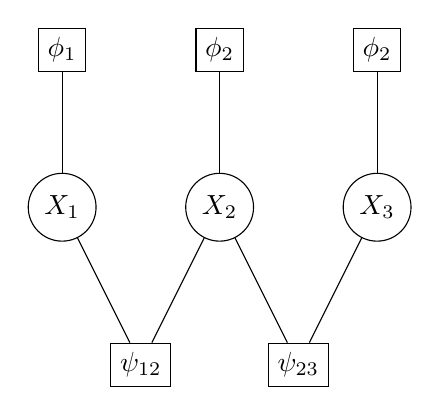
\begin{tikzpicture}[var/.style={circle,draw},factor/.style={rectangle,draw}]
\node[var] (x1) at (0,0) {$X_1$}; 
\node[var] (x2) at (2,0) {$X_2$};
\node[var] (x3) at (4,0) {$X_3$};
\node[factor] (u1) at (0,2) {$\phi_1$};
\node[factor] (u2) at (2,2) {$\phi_2$};
\node[factor] (u3) at (4,2) {$\phi_2$};
\node[factor] (p12) at (1,-2) {$\psi_{12}$};
\node[factor] (p23) at (3,-2) {$\psi_{23}$};
\path (x1) edge (u1); \path (x2) edge (u2); \path (x3) edge (u3);
\path (x1) edge (p12); \path (x2) edge (p12);
\path (x2) edge (p23); \path (x3) edge (p23);
\end{tikzpicture}\caption{Simple factor graph with $3$ variables, unary and pairwise factors.}
\end{figure}

\end{example}

In summary, factor graphs not only unify the representation of directed and undirected models but also provide the natural stage on which message-passing inference algorithms operate. For this reason, they will serve as a central tool in later chapters when we study inference in Markov random fields and its application to combinatorial optimization problems.

\paragraph{Canonical over-complete representation.}
For discrete graphical models, an equivalent but often more convenient parameterization is obtained through the canonical over-complete representation. Rather than associating features with a minimal set of sufficient statistics, one introduces indicator functions for every local assignment of each variable and factor. For a factor graph with variables $X_i \in \mathcal{X}_i$ and factors $F \in \mathcal{F}$, the unary sufficient statistics are
\begin{equation}
\phi_{i,y}(x)=\mathbbm{1}\{x_i=y\}, \qquad y\in\mathcal{X}_i,
\end{equation}
while the factor sufficient statistics are
\begin{equation}
\phi_{\FACTOR,y_{\FACTOR}}(\XVEC)=\mathbbm{1}\{\XFACT=y_{\FACTOR}\}, \qquad y_{\FACTOR}\in\mathcal{X}_{\FACTOR} .
\end{equation}
The corresponding exponential-family distribution can then be written as
\begin{equation}
p_{\EPARAM}(\XVEC)
=
\exp\left(
\sum_{i\in \VCGV}\sum_{y\in\mathcal{X}_i}\EPARAM_{i,y}\phi_{i,y}(\XVEC)
+
\sum_{\FACTOR\in\FACTORSET}\sum_{y_{\FACTOR}\in\mathcal{X}_{\FACTOR}}
\theta_{\FACTOR,y_{\FACTOR}}\phi_{\FACTOR,y_{\FACTOR}}(\XVEC)
-
A(\theta)
\right).
\end{equation}
This representation is called over-complete because the indicator statistics are linearly dependent: for each variable or factor, exactly one local configuration is active, so the associated indicators sum to one. Consequently, the natural parameters are not identifiable without additional constraints or gauge choices. Nevertheless, the over-complete form is particularly useful for graphical models because it aligns directly with local potentials, marginal inference, and variational relaxations. In this parameterization, learning can still be interpreted as moment matching, but the moments now correspond to unary and factor marginals. Approximate inference algorithms such as belief propagation therefore naturally operate on these quantities, returning beliefs $\mu_i(\XVEC_i)$ and $\mu_{\FACTOR}(x_{\FACTOR})$ that approximate the marginal expectations of the corresponding indicator sufficient statistics \cite{wainwright_graphical_2007}. When we refer to \emph{over-complete parameters}, we mean natural parameters whose entries are indexed by this over-complete set of indicator sufficient statistics. Thus, over-completeness is formally a property of the sufficient-statistic representation, not of the parameters themselves; the parameters are called over-complete only as shorthand for being compatible with that representation.


\subsection{Inference and Belief Propagation}
In graphical models, \emph{inference} refers to the set of tasks through which one extracts useful probabilistic information from a factorized distribution. The most common forms are: computing marginal distributions of individual variables or subsets of variables, estimating conditional probabilities given evidence, evaluating the partition function, and solving for the maximum a posteriori (MAP) configuration. Each of these problems is central to applications of Markov Random Fields: marginals provide uncertainty estimates, the partition function controls normalization and likelihood evaluation, and MAP inference directly corresponds to combinatorial optimization by identifying the lowest-energy configuration.

Exact inference is only tractable for models with restricted structure, such as trees or graphs with small treewidth. For general graphs, marginal inference and partition function computation are \#P-hard, while MAP inference is NP-hard \citep{chandrasekaran_complexity_2008,schrijver_combinatorial_2003}. As a result, research has focused on approximate inference algorithms. Two major families dominate: sampling-based approaches such as Markov Chain Monte Carlo \citep{geman_stochastic_1984} and deterministic algorithms based on variational approximations \citep{wainwright_graphical_2007}. Among the latter, message-passing algorithms are particularly appealing because they exploit the structure of factor graphs to perform distributed local computations.

\emph{Belief Propagation} (BP) is the canonical message-passing algorithm for inference in factor graphs. In its sum--product form, BP computes approximate marginal distributions by iteratively exchanging messages between variable nodes and factor nodes. In its max--product form, the algorithm approximates MAP inference by replacing summations with maximizations. On tree-structured graphs, both algorithms are exact and run in time linear in the number of edges, making BP highly efficient in this setting. On graphs with cycles, the same iterative procedure can still be applied; in this case it is known as \emph{loopy BP}. Although not guaranteed to converge, loopy BP often provides remarkably accurate approximations in practice and has been shown to correspond to stationary points of the Bethe free energy \citep{yedidia_understanding_2003}.

For this thesis, inference plays a dual role. On the one hand, it is the computational mechanism through which probabilistic quantities and approximate solutions to combinatorial problems are obtained. On the other hand, because many inference algorithms such as BP can be expressed as differentiable computational graphs, they can be embedded into end-to-end trainable architectures. This differentiability enables the backpropagation of gradients through the inference process, allowing parameters of neural networks or energy functions to be learned directly by gradient descent. This approach stands in contrast to alternative methods such as MAP-perturbation techniques \citep{tarlow_randomized_2012,papandreou_perturb-and-map_2011,nowozin_perturb-and-map_2014}, which approximate gradients indirectly via sampling perturbed MAP solutions. By leveraging differentiable inference, our work integrates the structure and interpretability of MRFs with the flexibility of modern deep learning, setting the stage for the contributions developed in later chapters.


\subsubsection{Sum--product BP (marginals)}
The sum--product algorithm, also known as Belief Propagation (BP), is a message-passing procedure for computing marginal distributions in factor graphs. Its central idea is that local computations on the bipartite structure of the factor graph can be combined to yield global information about the distribution. On tree-structured graphs, the algorithm is exact and runs in time linear in the number of edges; on graphs with cycles it becomes an approximation, known as \emph{loopy BP}, which nevertheless performs surprisingly well in many applications \citep{yedidia_understanding_2003,kschischang_factor_2001}.

Formally, let $H=(V\cup F,E_H)$ be a factor graph. Messages are passed iteratively along edges from variables to factors and from factors to variables:
\begin{align}
m_{i\rightarrow f}(x_i) &= \prod_{g\in N(i)\setminus\{f\}} m_{g\rightarrow i}(x_i),\\
m_{f\rightarrow i}(x_i) &= \sum_{x_{f\setminus i}} \psi_f(x_f)\prod_{j\in f\setminus i} m_{j\rightarrow f}(x_j).
\end{align}
Variable-to-factor messages represent the belief of a variable node about its state based on all other neighboring factors, while factor-to-variable messages aggregate information from neighboring variables mediated by the factor potential. Once messages have converged (or after a fixed number of iterations), approximate beliefs are computed as
\[
b_i(x_i)\propto \prod_{f\in N(i)} m_{f\rightarrow i}(x_i), \qquad 
b_f(x_f)\propto \psi_f(x_f)\prod_{i\in f} m_{i\rightarrow f}(x_i).
\]
These beliefs approximate marginal distributions for nodes and factors. On trees, they coincide exactly with the true marginals.

\begin{algorithm}[htbp]
\caption{Sum--product Belief Propagation}
\KwData{Factor graph $H=(V\cup F,E_H)$, messages $\{m\}$}
\KwResult{Approx.\ beliefs $\{b_i,b_f\}$}
Initialize all messages (e.g., uniformly);\;
\Repeat{convergence or max-iter}{
\ForEach{$(i,f)\in E_H$}{
Update $m_{i\to f}$ and $m_{f\to i}$ according to the update equations.}}
Compute beliefs $b_i, b_f$ from messages.\;
\end{algorithm}

The sum--product algorithm can be interpreted from multiple perspectives. It arises naturally as dynamic programming on trees, as variational optimization of the Bethe free energy \citep{yedidia_understanding_2003}, and as exact marginalization in factor graphs of bounded treewidth. In loopy graphs, fixed points of the message updates correspond to stationary points of the Bethe free energy, providing a variational justification for its use. From a computational viewpoint, the algorithm distributes the intractable global inference task into many local updates, each involving only small subsets of variables. This locality makes BP highly scalable and parallelizable, which explains its widespread use in areas such as error-correcting codes, computer vision, and structured prediction in machine learning.

In the context of this thesis, the sum--product algorithm is important not only as a classical inference method but also because its iterative updates are differentiable operations. This property allows BP to be unrolled and integrated into neural architectures, enabling backpropagation of gradients through the inference process. By embedding differentiable BP into training, we can jointly optimize parameters of energy functions and neural networks while respecting the graphical structure of the problem.


\paragraph{Max--product BP (MAP)}
Replacing $\sum$ by $\max$ (and products by sums in log domain) yields max--product; on trees it recovers dynamic programming for MAP. On loopy graphs, convergence is not guaranteed; convex variants such as tree-reweighted message passing (TRW/ TRW-S) provide bounds and convergence guarantees for specific energies \citep{kolmogorov_convergent_2006}.


\subsubsection{When and why does BP work?}
Belief Propagation is exact on trees, but on graphs with cycles its behavior is more subtle. Empirically, loopy BP has been found to give high-quality approximations in many applications, from error-correcting codes to computer vision, even when theoretical guarantees are lacking. Understanding the regimes in which BP provides correct results has therefore been an important line of research.

Beyond trees, BP is known to provably solve certain classes of combinatorial optimization problems. For example, it exactly recovers maximum-weight matchings and $b$-matchings under appropriate conditions \citep{bayati_maximum_2005, huang_loopy_2007, bayati_belief_2011, shin_graphical_2013}, and can solve instances of min-cost flow \citep{gamarnik_belief_2012}. These results demonstrate that, despite its heuristic nature in loopy graphs, BP can coincide with exact combinatorial algorithms in structured settings. On the practical side, distributed and parallel implementations \citep{gonzalez_parallel_2010, ma_task_2012} allow BP to scale to very large graphs, making it attractive in network and graph mining applications.

It is also worth clarifying terminology: the \emph{sum--product} algorithm is used for computing marginals, while the \emph{max--product} algorithm is its counterpart for MAP inference. The latter is often implemented in log-space, in which case products of probabilities become sums of log-probabilities, yielding the so-called \emph{max--sum} algorithm. The two names thus refer to the same underlying procedure, with max--sum being a numerically more stable implementation. This distinction helps to situate BP within the broader family of dynamic programming methods such as the Viterbi algorithm, which also operates in the max--sum (log-space) domain.

Despite these successes, BP also has well-documented limitations. On loopy graphs, it may fail to converge or converge to poor fixed points. Techniques such as damping, residual scheduling, and convex free-energy approximations can mitigate these issues but do not eliminate them entirely \citep{yedidia_understanding_2003, kolmogorov_convergent_2006}. Furthermore, when factors involve many variables or when variables have large alphabets, the size of messages becomes prohibitive. In such cases, structured factors and low-rank approximations can be used in practice to reduce complexity \citep{wainwright_graphical_2007}.


\subsubsection{Learning-augmented Belief Propagation}
While classical BP is purely algorithmic and determined by the graphical model structure and its potentials, recent research has explored how learning can be used to augment or modify the BP procedure itself. The motivation is twofold: first, to overcome some of the limitations of standard BP, such as poor convergence or inaccurate marginals on loopy graphs; and second, to integrate inference more tightly with modern machine learning pipelines where parameters are trained end-to-end.

Learning can intervene at several levels of the BP algorithm. One approach is to make the \emph{messages} themselves parametric and learnable, so that instead of strictly following the sum--product or max--product updates, neural networks predict or reweight the messages passed along edges. This idea underlies neural message-passing architectures that generalize BP by embedding richer computations within each update \citep{satorras_neural_2021}. A second approach is to learn the \emph{message schedule}, i.e., the order and frequency with which messages are updated. By training update schedules on data, convergence speed and accuracy can often be improved relative to fixed synchronous or asynchronous schemes. A third line of work uses learning to adapt the \emph{potentials} of the graphical model itself, either by parameterizing them with neural networks or by amortizing inference across many instances of a problem class \citep{wiseman_amortized_2019}.

These developments fall under the broader paradigm of \emph{learning to infer}, where inference algorithms are not treated as fixed black boxes but as differentiable computational graphs whose parameters can be optimized from data. Differentiable BP variants allow gradients to be propagated through the inference process, enabling neural networks to be trained with feedback that depends on approximate marginals or MAP configurations. This sets them apart from sampling-based gradient estimators or MAP-perturbation methods \citep{tarlow_randomized_2012,nowozin_perturb-and-map_2014}, which do not permit exact backpropagation.



\begin{figure}[htbp]
\centering
\begin{tikzpicture}[node distance=2cm, every node/.style={font=\small}]
  % Variable nodes
  \node[circle,draw,minimum size=0.8cm] (x1) {$x_1$};
  \node[circle,draw,minimum size=0.8cm, right of=x1] (x2) {$x_2$};
  \node[circle,draw,minimum size=0.8cm, right of=x2] (x3) {$x_3$};
  % Factor nodes
  \node[rectangle,draw,minimum width=0.9cm,minimum height=0.6cm,below of=x1,node distance=1.5cm] (f1) {$\psi_1$};
  \node[rectangle,draw,minimum width=0.9cm,minimum height=0.6cm,below of=x2,node distance=1.5cm] (f2) {$\psi_{12}$};
  \node[rectangle,draw,minimum width=0.9cm,minimum height=0.6cm,below of=x3,node distance=1.5cm] (f3) {$\psi_2$};
  % Edges
  \draw (x1) -- (f1);
  \draw (x1) -- (f2);
  \draw (x2) -- (f2);
  \draw (x2) -- (f3);
  \draw (x3) -- (f3);
  % Neural annotation
  \node[below=0.8cm of f2,font=\footnotesize,align=center] (nn) {Neural module \\ adapting messages};
  \draw[->,dashed] (nn.north) -- (f2.south);
\end{tikzpicture}
\caption{Schematic illustration of learning-augmented Belief Propagation. 
Classical messages (solid edges) are complemented by neural modules (dashed arrow) that reweight or adapt updates.}
\end{figure}

In this thesis, learning-augmented BP will play a central role. We will exploit the differentiability of message passing to integrate it directly into our models for combinatorial optimization. By combining the structure and interpretability of BP with the flexibility of neural networks, we aim to design inference mechanisms that are both expressive and trainable, bridging the gap between classical graphical model inference and modern deep learning approaches.



\begin{example}{\hrule\vspace{.2em}BP on a chain (exact)\vspace{.2em}\hrule}
For a chain $X_1$--$X_2$--$X_3$ with unary and pairwise factors $\{\phi_1,\phi_2,\phi_3,\psi_{12}, \psi_{23}\}$. During belief propagation, messages are iteratively exchanged along the edges between variables and factors. Each variable sends a \emph{variable-to-factor} message $q_{i \to F}$ that summarizes its current belief based on all other connected factors, while each factor sends a \emph{factor-to-variable} message $r_{F \to i}$ encoding the compatibility of variable states given its neighboring messages. After several iterations, these messages converge toward consistent marginal or MAP estimates for the variables. This simple three-variable example illustrates the bidirectional flow of information that underlies both sum-product and max-product belief propagation.


\begin{figure}[htbp]\centering
\begin{tikzpicture}[
  >=Latex,
  var/.style={circle,draw,minimum size=18pt,inner sep=1pt},
  factor/.style={rectangle,draw,rounded corners=0pt,minimum width=16pt,minimum height=12pt,inner sep=2pt},
  graphedge/.style={line width=0.5pt},
  msgVF/.style={->,thick,blue!70,shorten <=2pt,shorten >=2pt},
  msgFV/.style={->,thick,red!70,shorten <=2pt,shorten >=2pt},
  msglabel/.style={font=\scriptsize,fill=white,inner sep=1pt}
]

% --- Nodes
\node[var]    (x1) at (0,0)   {$X_1$}; 
\node[var]    (x2) at (4,0)   {$X_2$};
\node[var]    (x3) at (8,0)   {$X_3$};
\node[factor] (u1) at (0,2)   {$\FACTOR_1$};
\node[factor] (u2) at (4,2)   {$\FACTOR_2$};
\node[factor] (u3) at (8,2)   {$\FACTOR_2$}; % keep as provided
\node[factor] (p12) at (2,-2) {$\FACTOR_{12}$};
\node[factor] (p23) at (6,-2) {$\FACTOR_{23}$};

% --- Undirected factor-graph edges
\path[graphedge] (x1) -- (u1);
\path[graphedge] (x2) -- (u2);
\path[graphedge] (x3) -- (u3);
\path[graphedge] (x1) -- (p12);
\path[graphedge] (x2) -- (p12);
\path[graphedge] (x2) -- (p23);
\path[graphedge] (x3) -- (p23);

% --- Message arrows (one iteration t)
% Unary factors
\draw[msgVF,bend left=28] (x1) to node[msglabel,pos=0.5] {$m_{1\rightarrow \FACTOR_1}$} (u1);
\draw[msgFV,bend left=28] (u1) to node[msglabel,pos=0.5] {$m_{\FACTOR_1\rightarrow 1}$} (x1);

\draw[msgVF,bend left=28] (x2) to node[msglabel,pos=0.5] {$m_{2\rightarrow \FACTOR_2}$} (u2);
\draw[msgFV,bend left=28] (u2) to node[msglabel,pos=0.5] {$m_{\FACTOR_2\rightarrow 2}$} (x2);

\draw[msgVF,bend left=28] (x3) to node[msglabel,pos=0.5] {$m_{3\rightarrow \FACTOR_2}$} (u3);
\draw[msgFV,bend left=28] (u3) to node[msglabel,pos=0.5] {$m_{\FACTOR_2\rightarrow 3}$} (x3);

% Pairwise factors: psi_12
\draw[msgVF,bend left=28] (x1) to node[msglabel,pos=0.5] {$m_{1\rightarrow \FACTOR_{12}}$} (p12);
\draw[msgFV,bend left=28] (p12) to node[msglabel,pos=0.5]   {$m_{\FACTOR_{12}\rightarrow 1}$} (x1);

\draw[msgVF,bend left=28] (x2) to node[msglabel,pos=0.5] {$m_{2\rightarrow \FACTOR_{12}}$} (p12);
\draw[msgFV,bend left=28] (p12) to node[msglabel,pos=0.5]   {$m_{\FACTOR_{12}\rightarrow 2}$} (x2);

% Pairwise factors: psi_23
\draw[msgVF,bend left=28] (x2) to node[msglabel,pos=0.5] {$m_{2\rightarrow \FACTOR_{23}}$} (p23);
\draw[msgFV,bend left=28] (p23) to node[msglabel,pos=0.5]   {$m_{\FACTOR_{23}\rightarrow 2}$} (x2);

\draw[msgVF,bend left=28] (x3) to node[msglabel,pos=0.5] {$m_{3\rightarrow \FACTOR_{23}}$} (p23);
\draw[msgFV,bend left=28] (p23) to node[msglabel,pos=0.5]   {$m_{\FACTOR_{23}\rightarrow 3}$} (x3);

% --- Legend
\begin{scope}[shift={(0.0,-4.1)}]
  %\node[align=left,anchor=west,font=\small] at (0,1.2) {Legend (messages in iteration $t$):};
  \draw[msgVF] (0,0.6) -- ++(1.1,0) node[right,black,font=\scriptsize] {variable--to--factor $\,m_{i\rightarrow F}^{(t)}$};
  \draw[msgFV] (0,0.1) -- ++(1.1,0) node[right,black,font=\scriptsize] {factor--to--variable $\,m_{F\rightarrow i}^{(t)}$};
\end{scope}

\end{tikzpicture}
\caption{Simple factor graph with $3$ variables, unary and pairwise factors, with belief-propagation messages shown (blue: $m_{i\rightarrow \FACTOR}$, red: $m_{\FACTOR \rightarrow i}$).}
\label{fig:bp_message_passing}
\end{figure}

\end{example}


